\documentclass{article}
\usepackage{amsmath}
\usepackage[utf8]{inputenc} 
\usepackage{listings}
\usepackage{mathpazo}
\usepackage{tcolorbox}
\usepackage{xcolor}
\usepackage{graphicx}
\usepackage{multicol}

\title{Prosjekt i molekylar dynamik}
\author{Mia Synnøve Frivik}
\date{usikkert}

\begin{document}
\maketitle
\newpage
\section*{Oppgave 1}
a) 
\begin{figure}[h!]
 \centering
  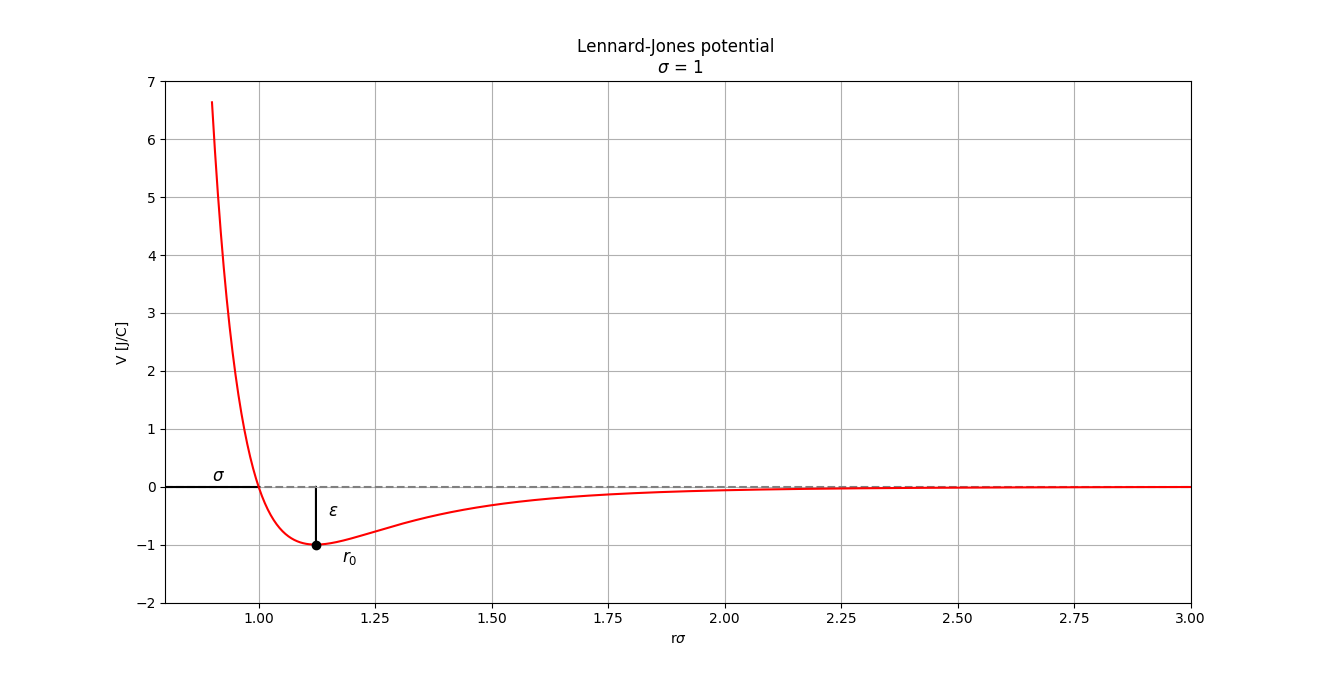
\includegraphics[width=0.80\textwidth]{Figure_1.png}
  \caption{}
\end{figure}

ser på formelen for Lennard-Jones potensialet $U(r) = 4\epsilon ((\frac{\sigma}{r})^{12} - (\frac{\sigma}{r})^6)$. Hvis $r < \sigma$, vil $r^{12}$ bli mindre enn $r^{6}$ noe som fører til at $(\frac{\sigma}{r})^{12} > (\frac{\sigma}{r})^6$. Det medfører at $U(r)$ blir positivt og at det er den frastøttende kraften som dominerer. Hvis $r > \sigma$, vil $r^{12}$ bli større enn $r^6$, altså vil $(\frac{\sigma}{r})^{12} < (\frac{\sigma}{r}^6)$. Det betyr at $U(r)$ blir negativt og det er da den tilltrekkende kraften som dominerer. I punkt $r_{0}$ (se Figur 1) vil den frastøttende kraften og den tiltrekkende kraften være like og er da i likevekt. Dette punktet er karakterisert som det punktet hvor den potensielle energien er lavest.\\
\\
La oss nå se på hva som skjer med to argon-atomer som ligger i en avstand $ 1.5 \sigma$fra hverandre som ilustrert i figur 2   
\begin{figure}[h!]
 \centering
  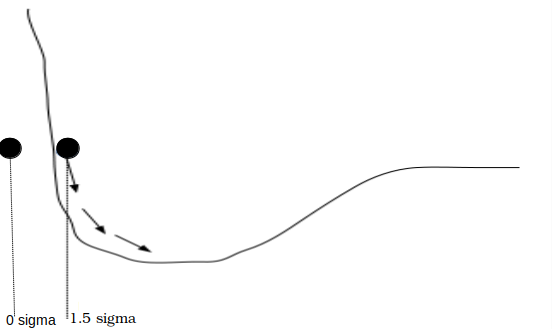
\includegraphics[width=50mm, scale=0.01]{Bilde_2.png}
  \caption{Feil fordi det egentlig skulle være sigma 0.95 på denne siden}
\end{figure}
\newpage
Hvis atomene starter med en avstand $1.5 \sigma$ vil avstande være stor nokk til at den tiltrekkende kraften og den frastøttende kraften nullerhverandre ut og atomene står nesten stille. Derimot kan man se at når avstanden er på $0.95  \sigma$ vil atomet ha nok energi til å unnslippe potensialbrønnen.

1b)
(i)\\
\begin{figure}[h!]
 \centering
  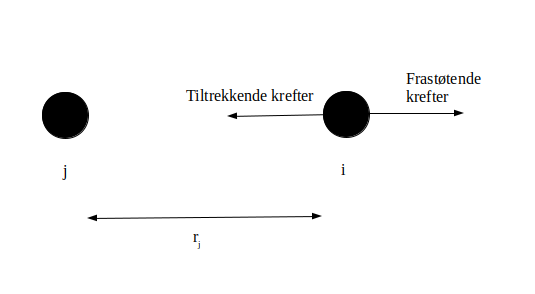
\includegraphics[width=0.80\textwidth]{Figur_2.png}
  \caption{Kreftene som virker på atom i}
\end{figure}\\
(ii)\\
\begin{align*}
F = -\frac{\partial u}{\partial r}
\end{align*}
(ii)\\
\begin{align*}
U(r) &= 4\epsilon((\frac{\sigma}{r})^12 - (\frac{\sigma}{r})^6)\\
\end{align*}
vet at $\vec{F} = -\frac{dU}{d\vec{r}} \cdot \frac{\vec{r}}{|\vec{r}|}$, man må gange med enhetsvektoren fordi kraften har en retning det har ikke potensiell energi.\\ så for å utlede ligningen for akselerasjon ser vi først på ligningen for et atom:
\begin{align*}
F &= (4\epsilon((\frac{\sigma}{r})^(12) - (\frac{\sigma}{r})^6))'\\
&= -4\epsilon(-12\frac{\sigma^12}{r^13} - (-6)\frac{\sigma^6}{r^7}) \cdot \frac{\vec{r}}{|\vec{r}|}\\
&= -4\epsilon(-12 \frac{\sigma^12}{r \cdot r^12} + 6 \frac{\sigma^6}{r \cdot r^6}) \cdot \frac{\vec{r}}{|\vec{r}|}\\
&= -4\epsilon(\frac{1}{r}(-12(\frac{\sigma}{r})^12 + 6(\frac{\sigma}{r})^6)) \cdot \frac{\vec{r}}{r}\\
&= -4\epsilon(-6(2(\frac{\sigma}{r})^12 - (\frac{\sigma}{r})^6)) \cdot \frac{\vec{r}}{r^2}\\
&= 24\epsilon(2(\frac{\sigma}{r})^12 - (\frac{\sigma}{r})^6) \cdot \frac{\vec{r}}{r^2}
\end{align*}\\
Setter inn $r = |\vec{r_i} - \vec{r_j}|$:
\begin{align*}
F = 24\epsilon(2(\frac{\sigma}{|\vec{r_i} - \vec{r_j}|})^12 - (\frac{\sigma}{|\vec{r_i}- \vec{r_j}|})^6) \cdot \frac{\vec{r_i}- \vec{r_j}}{|\vec{r_i} - \vec{r_j}|^2} 
\end{align*}
Siden likningen beskriver bevegelsen til atomet kommer summetegnet fra at man må legge sammen posisjonen til atomet ved forskjellige tider slik at vi kan beskrive bevegelsen
\end{document}
